\documentclass[aspectratio=1610]{beamer}
\usepackage[T1]{fontenc}
\usepackage{MnSymbol,wasysym}
\usepackage{multicol}
\usepackage{latexsym}
\usepackage{extarrows}
\usepackage[most]{tcolorbox}
\usepackage[backend=biber,natbib=true,style=authoryear, defernumbers=true]{biblatex}
%\usepackage[style=apa,backend=biber,natbib=true]{biblatex}
\usepackage{bookmark}
\usepackage{animate}
\usepackage[brazil]{babel}
\usepackage{media9}
%\bibliography{citacoes.bib}
\usetheme{wildcat}

\addbibresource{citacoes.bib}

\title{Desenvolvimento de aplicativo em Shiny para Visualização de Dados Meteorológicos no Rio Grande do Sul}
\date{\today}
\author{Pedro Dresseno John, Yuri Dessimon, Márcia Barbian}

% You change the titlegraphic to whatever you want, or comment it out to remove it.
%\titlegraphic{
\includegraphics[width=8cm]{3logos.png}}

\begin{document}

\begin{frame}
    \vspace{0.5cm}
    
\includegraphics[width=8cm]{3logos.png}
    \vspace{-2.5cm}
    \titlepage
\end{frame}

% \begin{frame}{Table of Contents}
%     \tableofcontents
% \end{frame}

\begin{frame}{O que é um \textit{shiny}?}
    \begin{itemize}
        \item Pacote de \textit{R} que permite fazer sites dinâmicos com código de \textit{R}
    \end{itemize}
    \animategraphics[autoplay,loop,width=0.8\linewidth]{6}{shiny_basico/shiny_basico-}{0}{64}
\end{frame}

\begin{frame}{Porque usar \textit{shiny}?}
    \begin{itemize}
        \item É bonito \smiley{} \pause
        \item Permite mostrar as relações entre muitas variáveis \pause
        \item Facilmente \textit{hosteável} na internet \pause
        \item Impressiona muito as pessoas (principalmente professores \& colegas)
    \end{itemize}
\end{frame}

\begin{frame}{Estrutura básica de um \textit{shiny}}
    \begin{itemize}
        \item \textit{ui} - \textit{user interface} (Interface de Usuário) \pause
        \item \textit{server} (Servidor) \pause
    \end{itemize}

    \begin{center}
        $$\huge{\textit{ui} \Longrightarrow \textit{server} \Longrightarrow \textit{ui}}$$
    \end{center}

    \pause

    \begin{columns}
        \begin{column}{0.333\textwidth}
            \begin{tcolorbox}[title=Passo 1: \textit{ui},height=5cm,colback=wcprimary10,colbacktitle=wcprimary,colframe=white,fontlower=\small]
                \small{
                Recebe os valores que o usuário coloca nos botões, calendários, caixas de texto, etc. e os coloca em um objeto chamado \textit{input} que é enviado ao servidor
                }
                \vfill
            \end{tcolorbox}    
        \end{column}
        
        \pause
        \begin{column}{0.333\textwidth}
            \begin{tcolorbox}[title=Passo 2: \textit{server},height=5cm,colback=wcprimary10,colbacktitle=wcprimary,colframe=white,fontlower=\small]
                \small{
                Recebe o objeto \textit{input}, e renderiza os gráficos, objetos de javascript ou até textos, e os coloca em um objeto chamado \textit{output}, que é enviado a interface de usuário novamente
                }
                \vfill
            \end{tcolorbox}    
        \end{column}
        
        \pause
        \begin{column}{0.333\textwidth}
            \begin{tcolorbox}[title=Passo 3: \textit{ui},height=5cm,colback=wcprimary10,colbacktitle=wcprimary,colframe=white,fontlower=\small]
                \small{
                Recebe o objeto final de \textit{output} e mostra o que o servidor renderizou ao usuário
                }
                \vfill
            \end{tcolorbox}    
        \end{column}
    \end{columns}
\end{frame}

\begin{frame}{Dados INMET - A maneira difícil}
    \begin{itemize}
        \item Os dados originalmente foram retirados manualmente das tabelas listadas no site do INMET: \href{https://tempo.inmet.gov.br/TabelaEstacoes/A001}{Dados das Estações}
    \end{itemize}
    \animategraphics[autoplay,loop,width=0.8\linewidth]{8}{tabela_inmet/tabela_inmet-}{0}{200}
\end{frame}

\begin{frame}{Dados INMET - A maneira fácil}
    \begin{itemize}
        \item O INMET tem um acervo histórico que permite baixar dados agregados anualmente de todas as estações simultaneamente: \href{https://portal.inmet.gov.br/dadoshistoricos}{Dados Históricos}
        \item O banco também vem já com todas as estações agregadas
    \end{itemize}
    \animategraphics[autoplay,loop,width=0.8\linewidth]{6}{dados_historicos/dados_historicos-}{0}{99}
\end{frame}

\begin{frame}{Variáveis do Banco}
    As observações são automáticamente feitas de hora em hora, normalmente com três versões: \textbf{Ins}, \textbf{Max} e \textbf{Min}
    \pause
    \begin{itemize}
        \item Temperatura (Cº)
        \begin{itemize}
            \item Ins, Max e Min
        \end{itemize}
        \pause
        \item Umidade (\%)
        \begin{itemize}
            \item Ins, Max e Min
        \end{itemize}
        \pause
        \item Ponto do Orvalho (C°)
        \begin{itemize}
            \item Ins, Max e Min
        \end{itemize}
        \pause
        \item Pressão (hPa)
        \begin{itemize}
            \item Ins, Max e Min
        \end{itemize}
        \pause
        \item \textbf{Vento} (m/s)
        \begin{itemize}
            \item Velocidade, Direção e Rajada
        \end{itemize}
        \pause
        \item \textbf{Radiação} (KJ/m)
        \pause
        \item \textbf{Chuva} (mm)
    \end{itemize}
\end{frame}

\begin{frame}{Página inicial do Aplicativo}
    Pacotes usados na ui: \textbf{shiny}, \textbf{shinyWidgets}, \textbf{shinydashboard}, \textbf{leaflet} e \textbf{plotly}
    Pacotes extras usados no servidor: \textbf{dplyr}, \textbf{htmltools}, \textbf{sp}, \textbf{sf}, \textbf{gstat}, \textbf{ggplot2}, \textbf{terra}, \textbf{leaflet.minicharts} e \textbf{leafsync}
    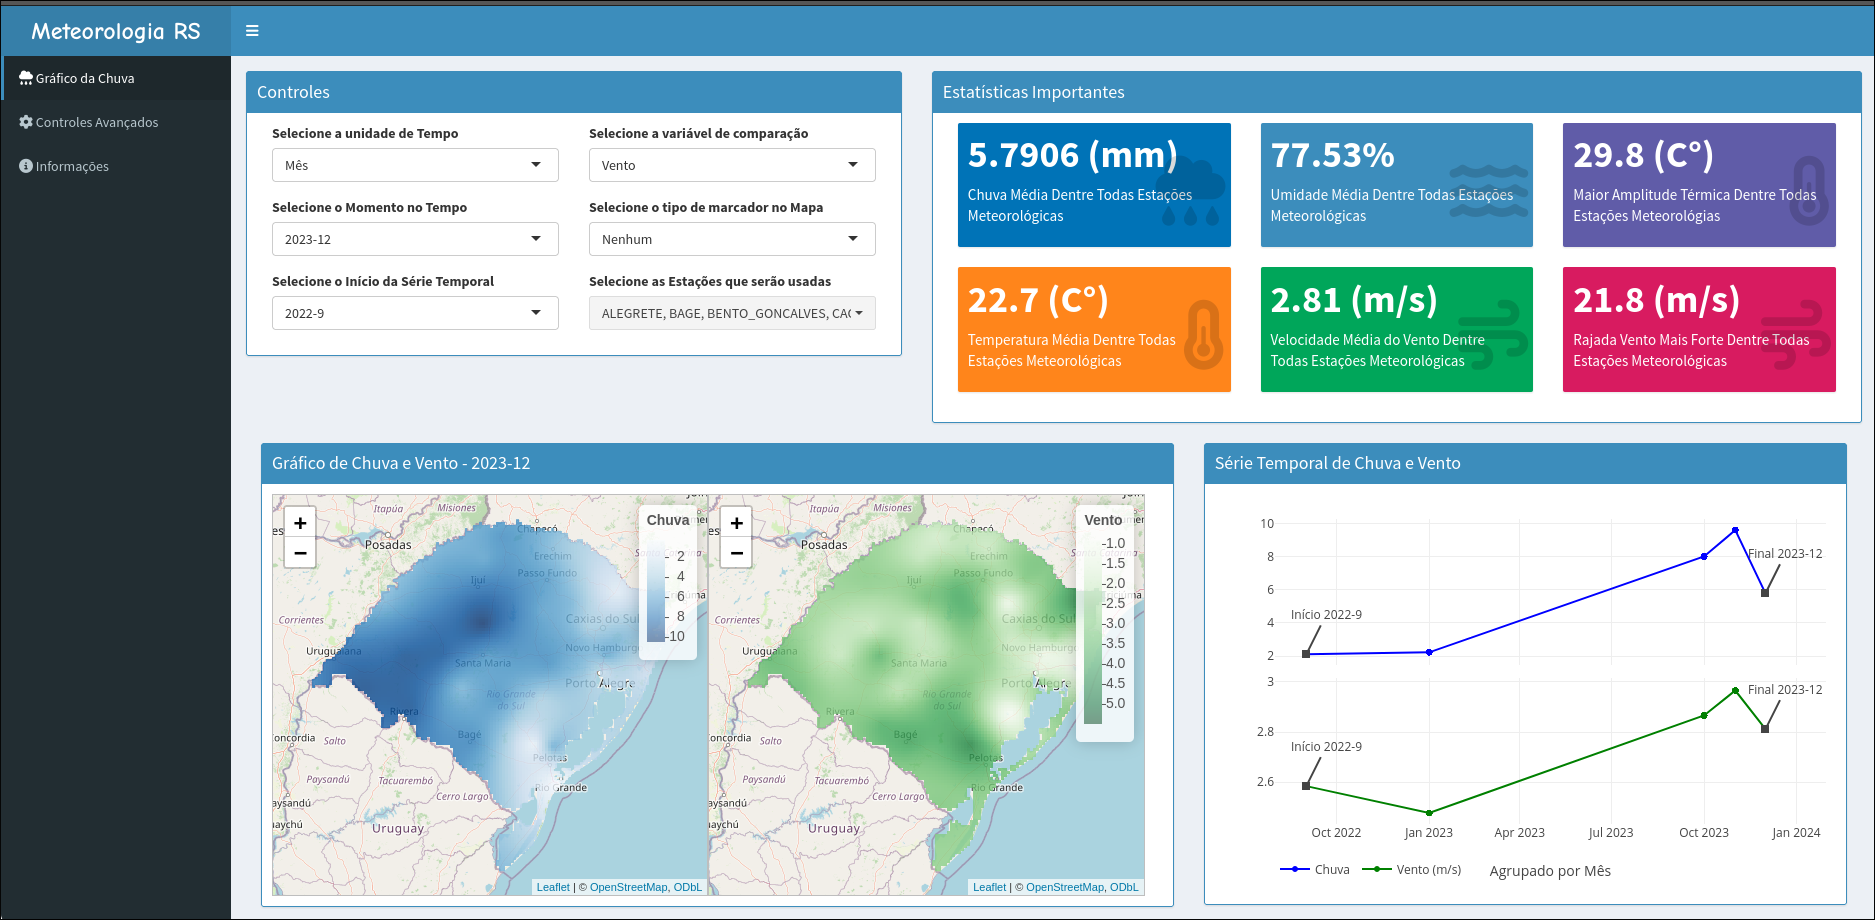
\includegraphics[width = \textwidth]{pagina_inicial.png}
\end{frame}

\begin{frame}{Tratamento do Banco - Antes do \textit{shiny}}
    Para que o banco fosse ideal para trabalhar no \textit{shiny} os seguintes passos foram feitos:
    \pause
    \begin{columns}    
        \begin{column}{0.5\textwidth}
            \begin{enumerate}
                \item Agrupar os dados que são observados de hora em hora, para criar quatro variáveis de data:
                \begin{itemize}
                    \item Dia
                    \item Semana
                    \item Mês
                    \item Ano
                \end{itemize}
                \pause
                \item Manualmente inserir a latitude e longitude baseada no nome da estação
                \pause
                \item Extrair o códgio da estação
            \end{enumerate}
        \end{column}
        \begin{column}{0.5\textwidth}
            \begin{tcolorbox}[title=dplyr \& shiny \& func. base,colback=wcprimary10,colbacktitle=wcprimary,colframe=white,fontlower=\small]
                \justify{
                    list.files()\newline
                    file.path()\newline
                    \%in\%\newline
                    switch()\newline
                    getElement()\newline
                    get()\newline
                    dplyr:rename()\newline
                    dplyr::select()\newline
                    dplyr::group\_by()\newline
                    dplyr::summarise()\newline
                    shiny::reactive()
                }
            \end{tcolorbox}
        \end{column}
    \end{columns}
\end{frame}

\begin{frame}{Shapefile e \textit{geobr}}
    \begin{itemize}
        \item Arquivo que nos dá o formato de uma região, seja estado, país, município, cidade, etc.
        \item No \textit{R} temos o pacote \textit{geobr} que permite carregar esses arquivos
    \end{itemize}
    \pause
    \begin{columns}
        \begin{column}{0.55\textwidth}
            \begin{tcolorbox}[title=Código,colback=wcprimary10,colbacktitle=wcprimary,colframe=white,fontlower=\small]
                \justify{
                    br = geobr::read\_country()\newline
                    regioes = geobr::read\_region()\newline
                    rs = geobr::read\_state("RS")\newline
                    mun = geobr::read\_municipality("RS")
                }
            \end{tcolorbox} 
        \end{column}
        \begin{column}{0.45\textwidth}
            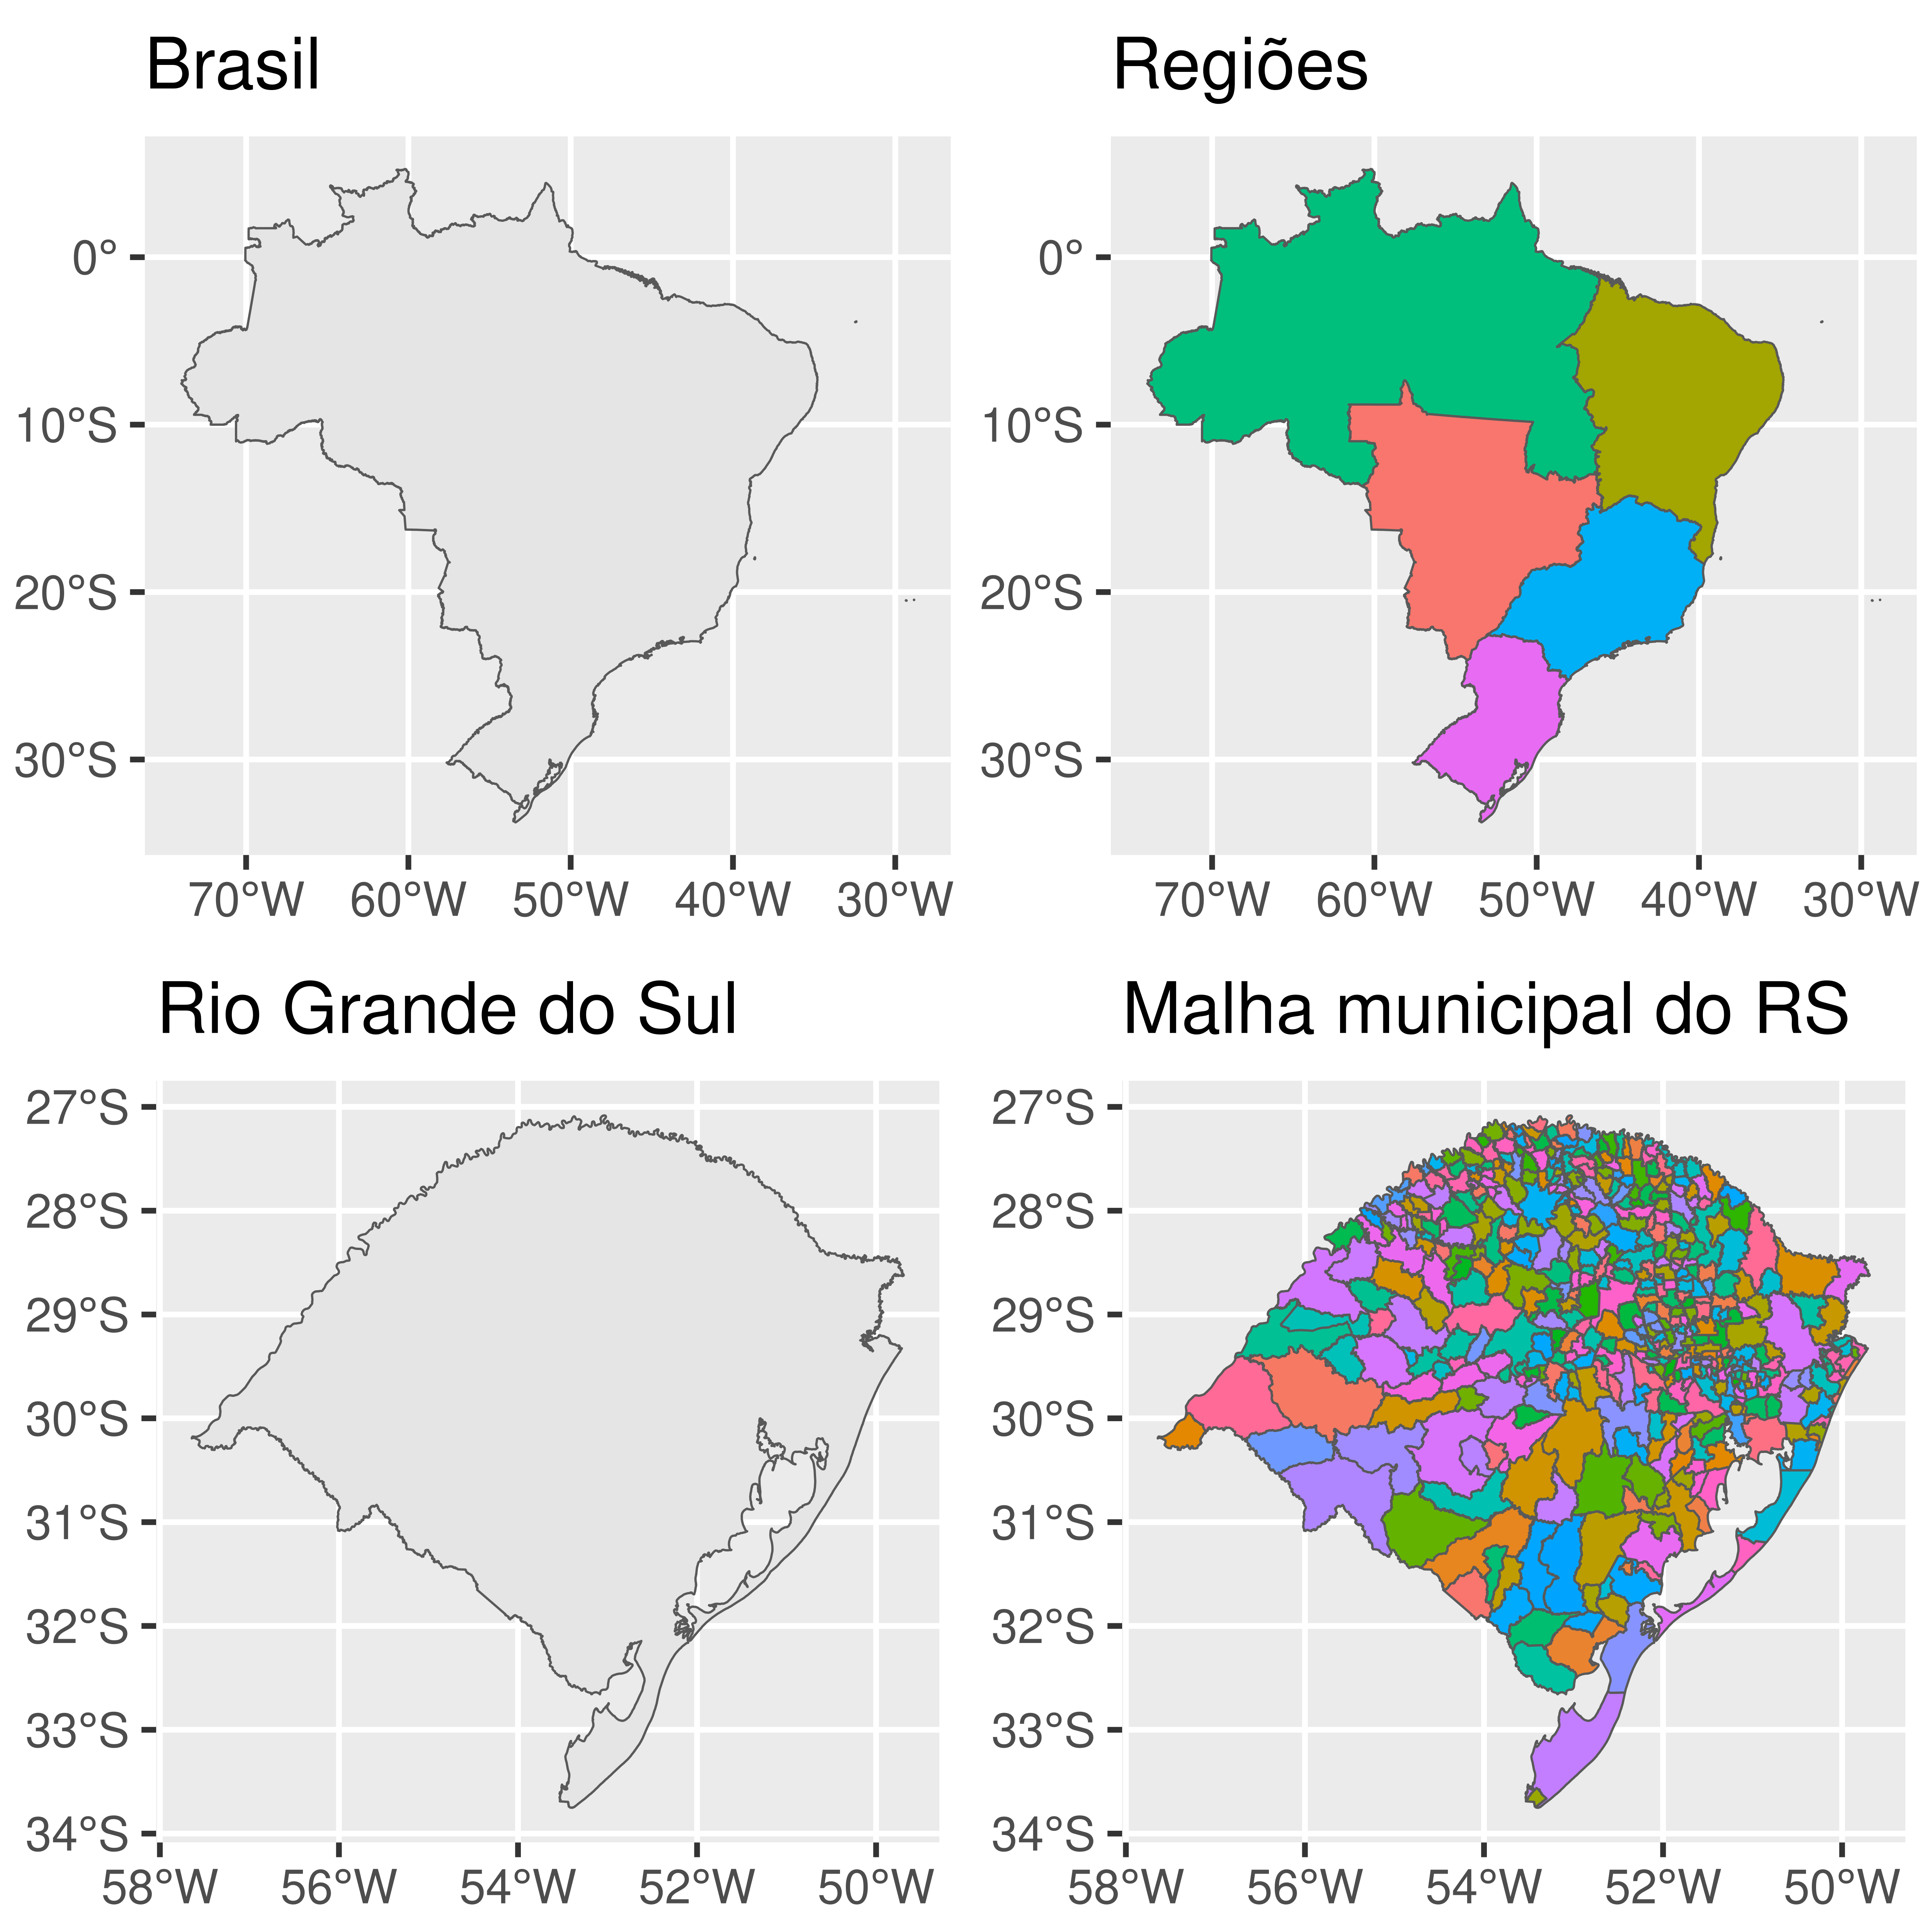
\includegraphics[width=\textwidth]{plots_geobr.png}
        \end{column}
    \end{columns}
\end{frame}

\begin{frame}{Controles do Aplicativo}
    Pode-se selecionar:
    \begin{columns}
        \begin{column}{0.5\textwidth}
            \begin{itemize}
                \item A unidade de tempo sendo usada \pause
                \item O momento no tempo a partir do qual a krigagem será feita \pause
                \item Uma data anterior para montagem de um gráfico de séries temporais \pause
                \item Uma variável para a krigagem secundária (dentre \textbf{Vento}, \textbf{Temperatura} ou \textbf{Umidade}) \pause
                \item A presença e tipo de marcador no mapa para as estações meteorológicas \pause
                \item Quais estações serão usadas ou excluídas
            \end{itemize}
        \end{column}
        \onslide<*>
        \begin{column}{0.5\textwidth}
            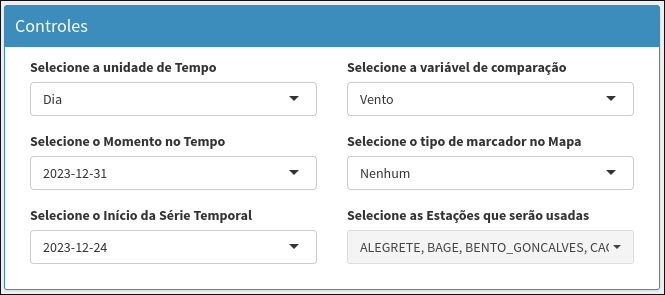
\includegraphics[width=\textwidth]{Controles.png}
            \begin{tcolorbox}[title=Código,colback=wcprimary10,colbacktitle=wcprimary,colframe=white,fontlower=\small]
                \justify{
                   shiny::selectInput() \newline
                   shinyWidgets::pickerInput()
                }
            \end{tcolorbox}
        \end{column}
    \end{columns}
\end{frame}

\begin{frame}{Value Boxes}
    Caixas coloridas com imagens e valores dinâmicos, muito bonitas.
    Presentes em vários pacotes, incluindo o \textbf{shinydashboard}.
    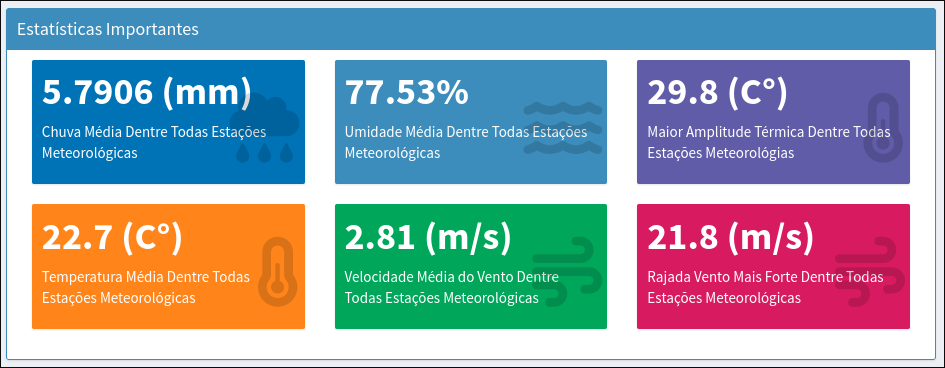
\includegraphics[width=\textwidth]{value_boxes.png}
\end{frame}

\begin{frame}{Gráfico de séries temporais}
    \begin{columns}
        \begin{column}{0.5\textwidth}
            \begin{itemize}
                \item ui reativa pro começo da série temporal
                \begin{itemize}
                    \item uiOutput
                    \item renderUI
                \end{itemize}
                \item \textit{plotly} ótimo pacote de gráficos
            \end{itemize}
            \begin{tcolorbox}[title=Código,colback=wcprimary10,colbacktitle=wcprimary,colframe=white,fontlower=\small]
                \justify{
                   plotly::plot\_ly()\newline
                   plotly::add\_trace()\newline
                   plotly::layout()\newline
                   plotly::layout(annotations = ...)\newline
                   plotly::subplot()\newline \newline
                   plotly::ggplotly()
                }
            \end{tcolorbox}
        \end{column}
        \begin{column}{0.5\textwidth}
            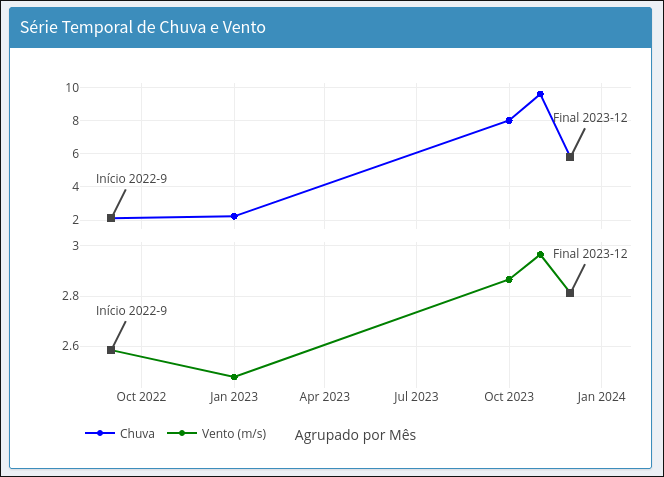
\includegraphics[width=\textwidth]{serie_temporal.png}
        \end{column}
    \end{columns}
\end{frame}

\begin{frame}{leaflet}
    Montando um gráfico do \textit{leaflet}
    \begin{columns}
        \begin{column}{0.5\textwidth}
            \begin{tcolorbox}[title=Código,colback=wcprimary10,colbacktitle=wcprimary,colframe=white,fontlower=\small]
                \justify{
                   |>\newline
                   leaflet::leaflet()\newline \pause
                   leaflet::addTiles()\newline \pause
                   leaflet::addRasterImage()\newline \pause
                   leaflet::addLegend()\newline \pause
                   leaflet::addMarkers()\newline \pause
                   leaflet.minicharts::addMinicharts()\newline\newline \pause

                   leaflet::setMaxBounds()
                }
            \end{tcolorbox}
        \end{column}
        \begin{column}{0.5\textwidth}
            \only<1>{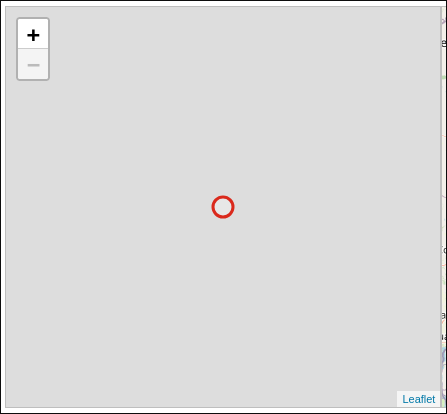
\includegraphics[width=\textwidth]{leaf.png}}
            \only<2>{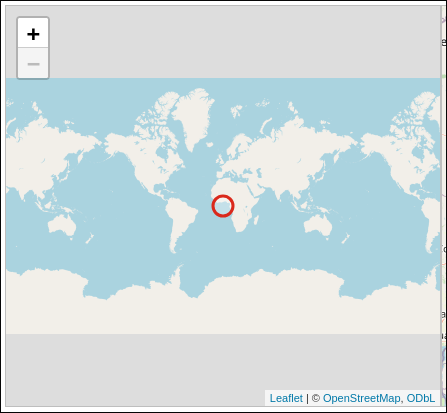
\includegraphics[width=\textwidth]{tiles.png}}
            \only<3>{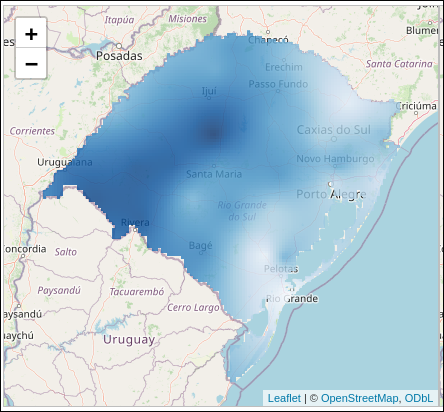
\includegraphics[width=\textwidth]{raster.png}}
            \only<4>{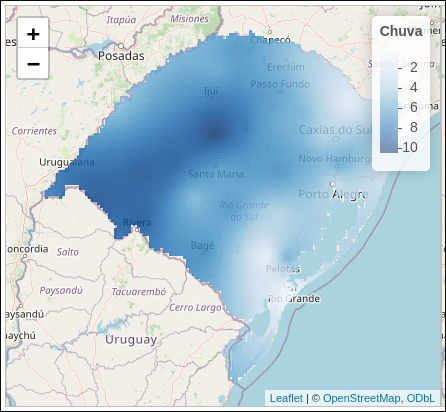
\includegraphics[width=\textwidth]{legend.png}}
            \only<5>{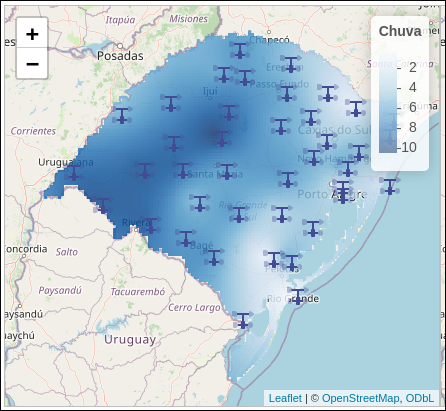
\includegraphics[width=\textwidth]{markers.png}}
            \only<6>{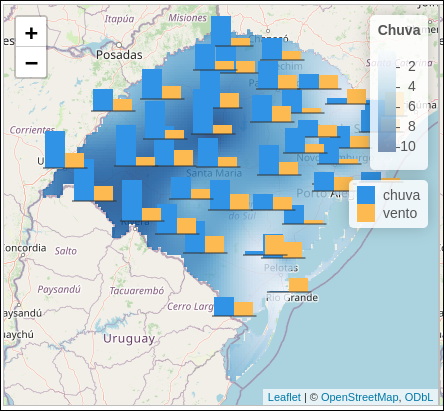
\includegraphics[width=\textwidth]{minicharts.png}}
            \only<7>{\animategraphics[autoplay,loop,width=1.1\linewidth]{6}{max_bounds/max_bounds-}{0}{61}}
        \end{column}
    \end{columns}
\end{frame}

\begin{frame}{leafsync}
    Útil para colocar dois ou mais gráficos do \textit{leaflet} juntos e também bem fácil de usar:
    \begin{columns}
        \begin{column}{0.5\textwidth}
            \begin{tcolorbox}[title=Código leafsync,colback=wcprimary10,colbacktitle=wcprimary,colframe=white,fontlower=\small]
                \justify{
                   mapa\_1 = leaflet::leaflet() |> ... \newline
                   mapa\_2 = leaflet::leaflet() |> ... \newline \newline

                   leafsync::sync(mapa\_1, mapa\_2)
                }
            \end{tcolorbox}
        \end{column}
        \begin{column}{0.5\textwidth}
            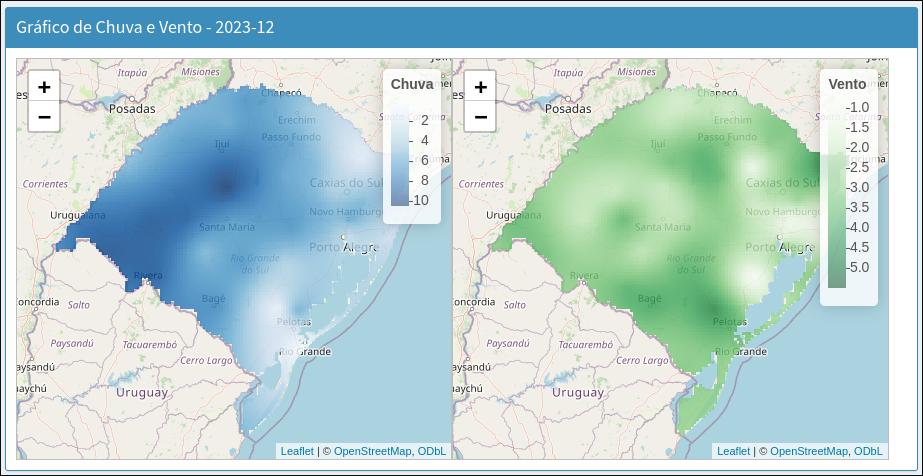
\includegraphics[width=\textwidth]{krigagem.png}
        \end{column}
    \end{columns}
\end{frame}

\begin{frame}{\Huge{GitHub}}
    \begin{columns}
        \begin{column}{0.4\textwidth}
            \Large{
                O código dessa apresentação e do aplicativo \textit{shiny} estão no GitHub
            }
            \newline
            \newline
            \Small{
            \href{https://github.com/johnpd4/apresentacao-rday5-2025}{https://github.com/johnpd4/apresentacao-rday5-2025}
            }
        \end{column}
        \begin{column}{0.5\textwidth}
            
\includegraphics[width=\textwidth]{qr_code.png}
        \end{column}
    \end{columns}
\end{frame}

\begin{frame}{Agradecimentos}
    \Large{Agradecemos à Fundação de Amparo à Pesquisa do Estado do Rio Grande do Sul (FAPERGS) pelo apoio financeiro, por meio do Projeto nº 24/2551-0002361-5, contemplado no Edital 06/2024 – Programa de Pesquisa e Desenvolvimento Voltado a Desastres Climáticos. Este suporte foi fundamental para a realização e o avanço desta pesquisa.}
\end{frame}

\begin{frame}[allowframebreaks]{Referências}
    \nocite{*}
    \printbibliography[heading=none]
\end{frame}

\standout{Obrigada!}

\end{document}